\chapter{Метод перехідної спектроскопії \\ локальних рівнів}\label{chapDLTS}
%\section{Еволюція комп'ютерних мереж}\label{sec101}

У 1974~р. Д.Ланг запропонував елегантний метод визначення параметрів дефектів дефектів,
який базується на вимірюваннях релаксації ємності бар'єрних структур після прикладання
імпульсу напруги \cite{Lang} .
Метод отримав назву перехідної спектроскопії локальних рівнів (deep--level transient spectroscopy, DLTS).
Фізичною передумовою методу є той факт, що ширина області просторового заряду в структурах Шотки чи $p$--$n$--переходах
залежить від прикладеної напруги, а отже змінюючи цю величину можна керувати положенням рівня Фермі в певному
прошарку матеріалу.

Розглянемо для визначеності контакт електронного напівпровідника з металом.
На рис.\ref{F21} представлена схема енергетичної діаграми такої структури при двох значеннях зворотної напруги $V$.
Поблизу межі розділу в напівпровіднику розташовується  збіднений шар,
тобто область зі зменшеною кількістю вільних носіїв заряду, яка виникла
внаслідок присутності електричного поля.
Її ширина визначається з умови
\begin{equation}
W=\left[\frac{2\varepsilon\varepsilon_0(V_{bi}+V)}{q^2N_D}\right]^{0.5}\,,
\end{equation}
де
$\varepsilon$ --- діелектрична проникність напівпровідника,
$\varepsilon_0$ ---діелектрична стала,
$V_{bi}$ --- контактна різниця потенціалів,
%$V$ ---прикладена до контакту зворотна напруга,
$N_D$ --- концентрація донорів,
$q$ --- елементарний заряд.

\begin{figure}[t]
\center
\vspace{-5mm}
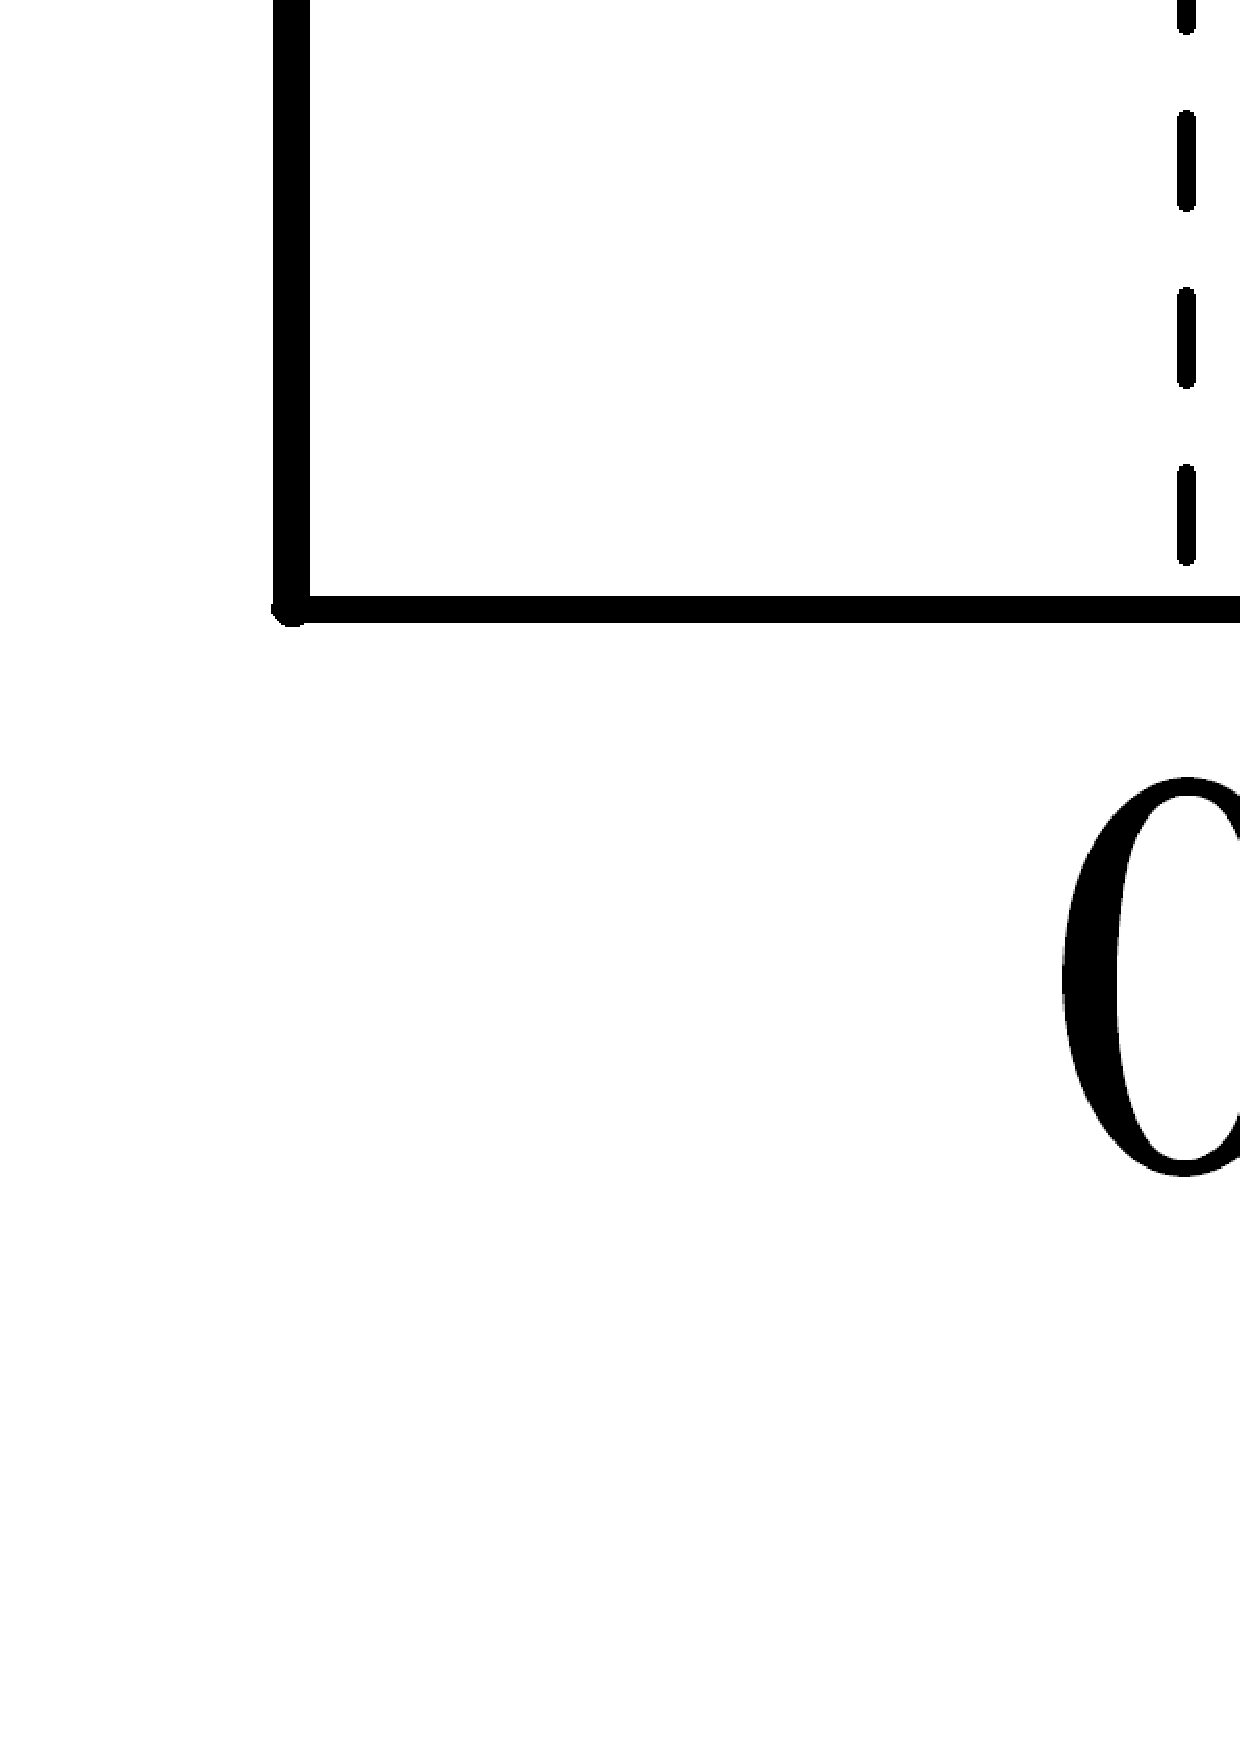
\includegraphics[width=0.6\textwidth]{Fig2_1}
\vspace{-3mm}
\caption{Зонна діаграма контакту Шотки при
різних значення зворотної напруги $V_0$ (а) та $V_1$ (б).
Вважається, що в області $x<0$ розташовано метал,
а при  $x>0$ --- $n$--напівпровідник.
$V_{bi}$ --- контактна різниця потенціалів,
$W_0$ та $W_1$ --- ширини області просторового заряду,
$d_0$ та $d_1$ --- координати межі між областями різного зарядового
стану дефекту.
}
\vspace{-3mm}
\label{F21}
\end{figure}

Припустимо, що у напівпровіднику є рівномірно розподілений по об'єму дефект з концентрацією $N_t$ , якому
відповідає глибокий рівень $E_t$.
Якщо в глибині напівпровідника $E_F>E_t$, а $(V_{bi}+V)>(E_C-E_t)$,
то в збідненому шарі буде проходити межа між  областями, де дефект перебуває у різних зарядових станах.
Відстань цієї межі від контакту можна оцінити за допомогою співвідношення
\begin{equation}
d=W-\left[\frac{2\varepsilon\varepsilon_0(E_F-E_t)}{q\,N_D}\right]^{0.5}=W-\lambda_d\,.
\end{equation}
Якщо звернутися до рис.\ref{F21}, то при $x>d$
рівень буде переважно заповненим, при $x<d$ --- вільним.

У збідненому шарі присутній просторовий заряд $Q$, викликаний в загальному випадку
як іонізованими донорними домішками
(вже нескомпенсованими вільними електронами, як це відбувається в глибині напівпровідника)
так і зарядженими дефектами.
Величина заряду залежить від прикладеної напруги і тому розглядають таке поняття як диференційна
ємність структури:
\begin{equation}
\label{DLTSC}
C=\frac{dQ}{dV}\,.
\end{equation}
У випадку, коли концентрація дефектів достатньо низька та їхнім внеском у $Q$ можна знехтувати
\begin{equation}
\label{DLTSCsh}
C=A\left[\frac{q\varepsilon\varepsilon_0\,N_D}{2(V_{bi}+V)}\right]^{0.5}\,,
\end{equation}
де
$A$ --- площа структури.

При зміні величини зворотної напруги (напр., від $V_0$ до $V_1$,
як це показано на рис.~\ref{F21},а та \ref{F21},б відповідно),
повинні зміститися як межа збідненого шару (від $W_0$ до $W_1$),
так межа розділу областей з різним зарядовим станом дефекту (від $d_0$ до $d_1$).
Якщо перший процес визначається перерозподілом
вільних носіїв заряду і відбувається достатньо швидко (за час порядку максвелівського часу релаксації),
то для реалізації другого необхідно, щоб всі дефекти, розташовані в прошарку
між $d_0$ та $d_1$ емітували електрони.
Цей процес значно повільніший і тому безпосередньо після зміни напруги
в системі може бути зафіксована ємність $\Delta C$ надлишкова, порівняно з рівноважним випадком, що
описується виразом (\ref{DLTSCsh}).
У випадку низької концентрації дефектів ($\Delta C\ll C$), а також за умови $(W_1-W_0)\ll W_1$,
цю величину можна оцінити за допомогою співвідношення \cite{tuomisto2019}
\begin{equation}
\label{DLTdelC}
\Delta C=\frac{N_t\,C_0}{2N_D}\left[1-\frac{2\lambda_d}{W}\left(1-\frac{C(V)}{C_0}\right)-\left(\frac{C(V)}{C_0}\right)^2\right]\,,
\end{equation}
де
$C_0=C(0)$.
При $C_0\gg C(V)$ вираз спрощується
\begin{equation}
%\renewcommand{\theequation}{\thechapter.\arabic{equation}*}
%\addtocounter{equation}{-1}
\label{DLTdelC*}
\Delta C=\frac{N_t\,C_0}{2N_D} \,.\tag{\ref{DLTdelC}\,$'$}
\end{equation}

%\begin{equation}
%\label{DLTSint}
%\int_{d_0}^{d_1}\frac{dC}{C}=-\int_{d_0}^{d_1}\frac{n(x)}{N_D\,W^2}x \,dx\,.
%\end{equation}

\begin{figure}[b]
\center
\vspace{-5mm}
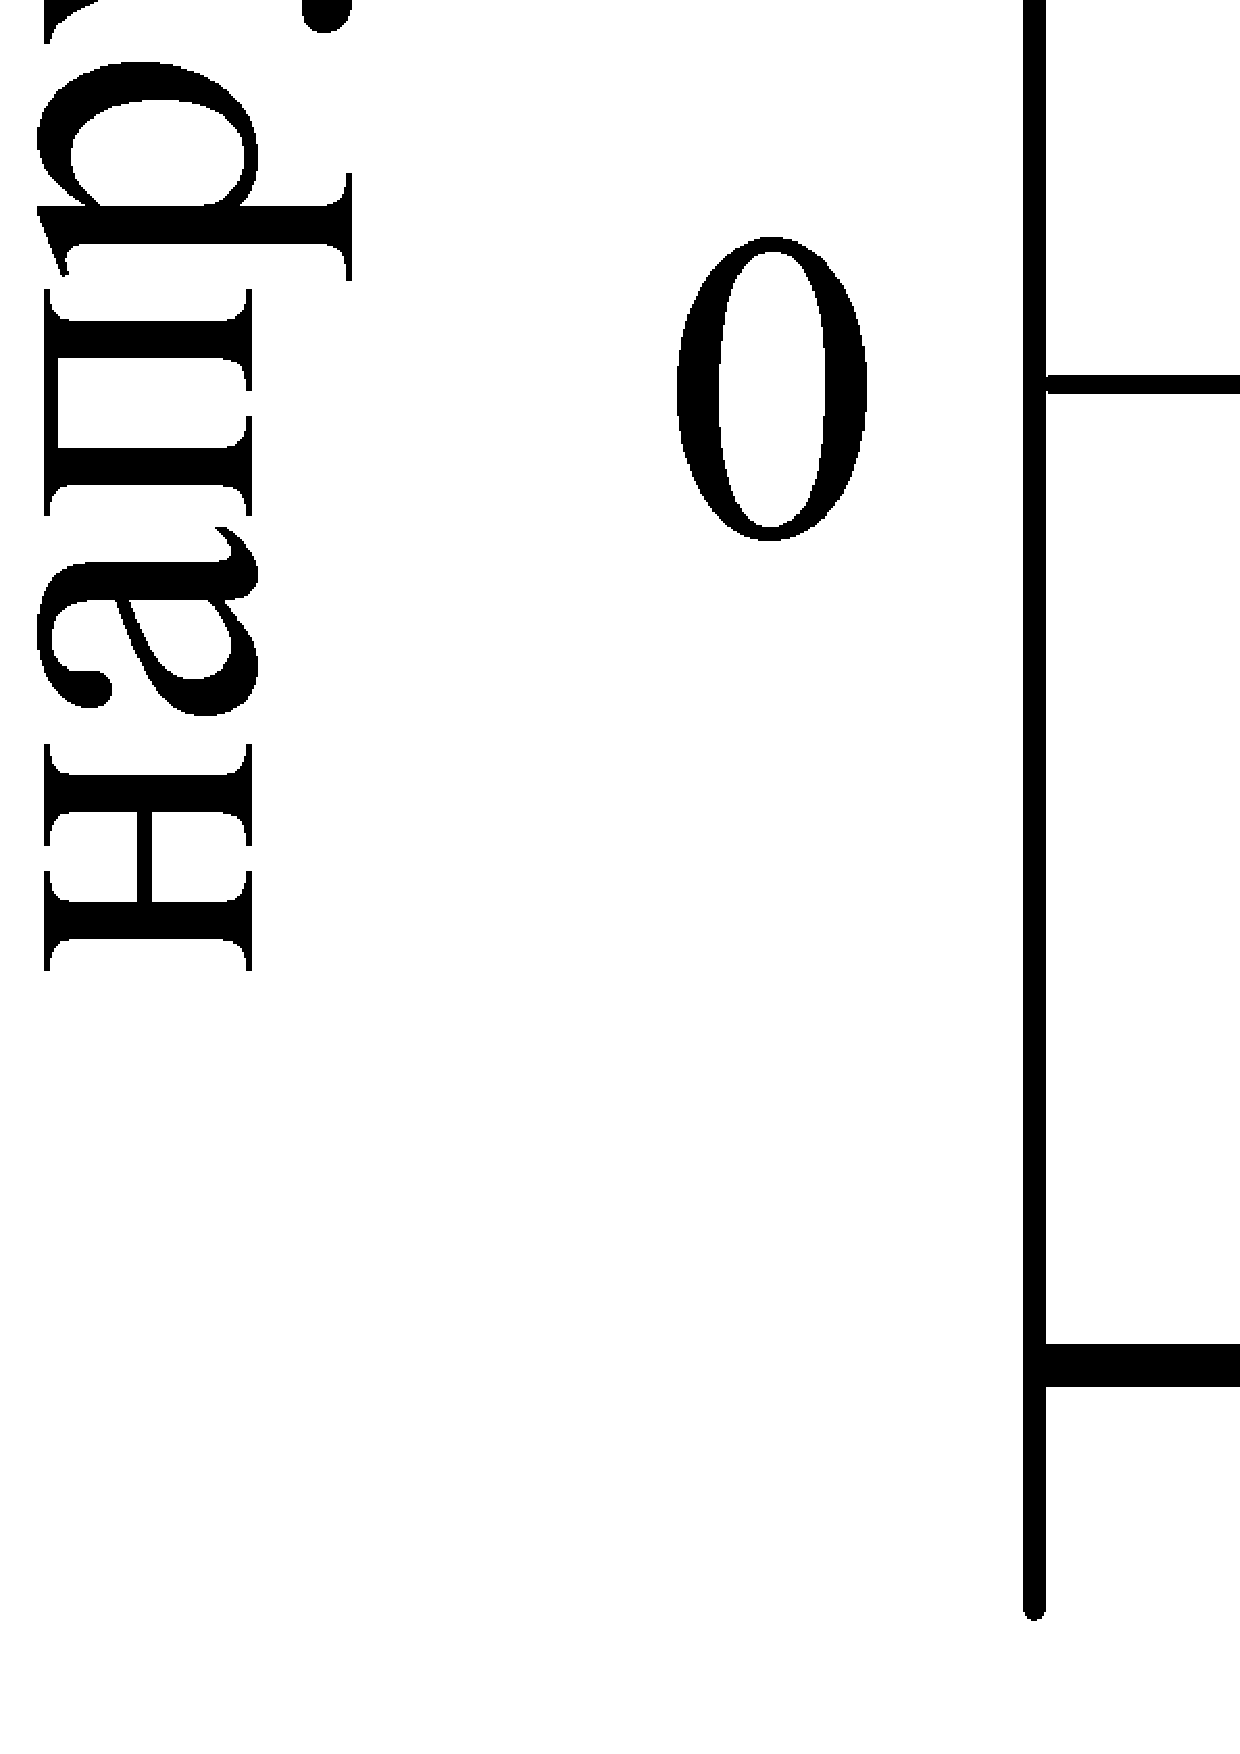
\includegraphics[width=0.6\textwidth]{Fig2_2}
\vspace{-3mm}
\caption{Режими зміщення бар'єрної структури в метод DLTS.
Кружечками позначено моменти виміру ємності.
}
\vspace{-3mm}
\label{F22}
\end{figure}


\begin{figure}[ht]
\center
\vspace{-5mm}
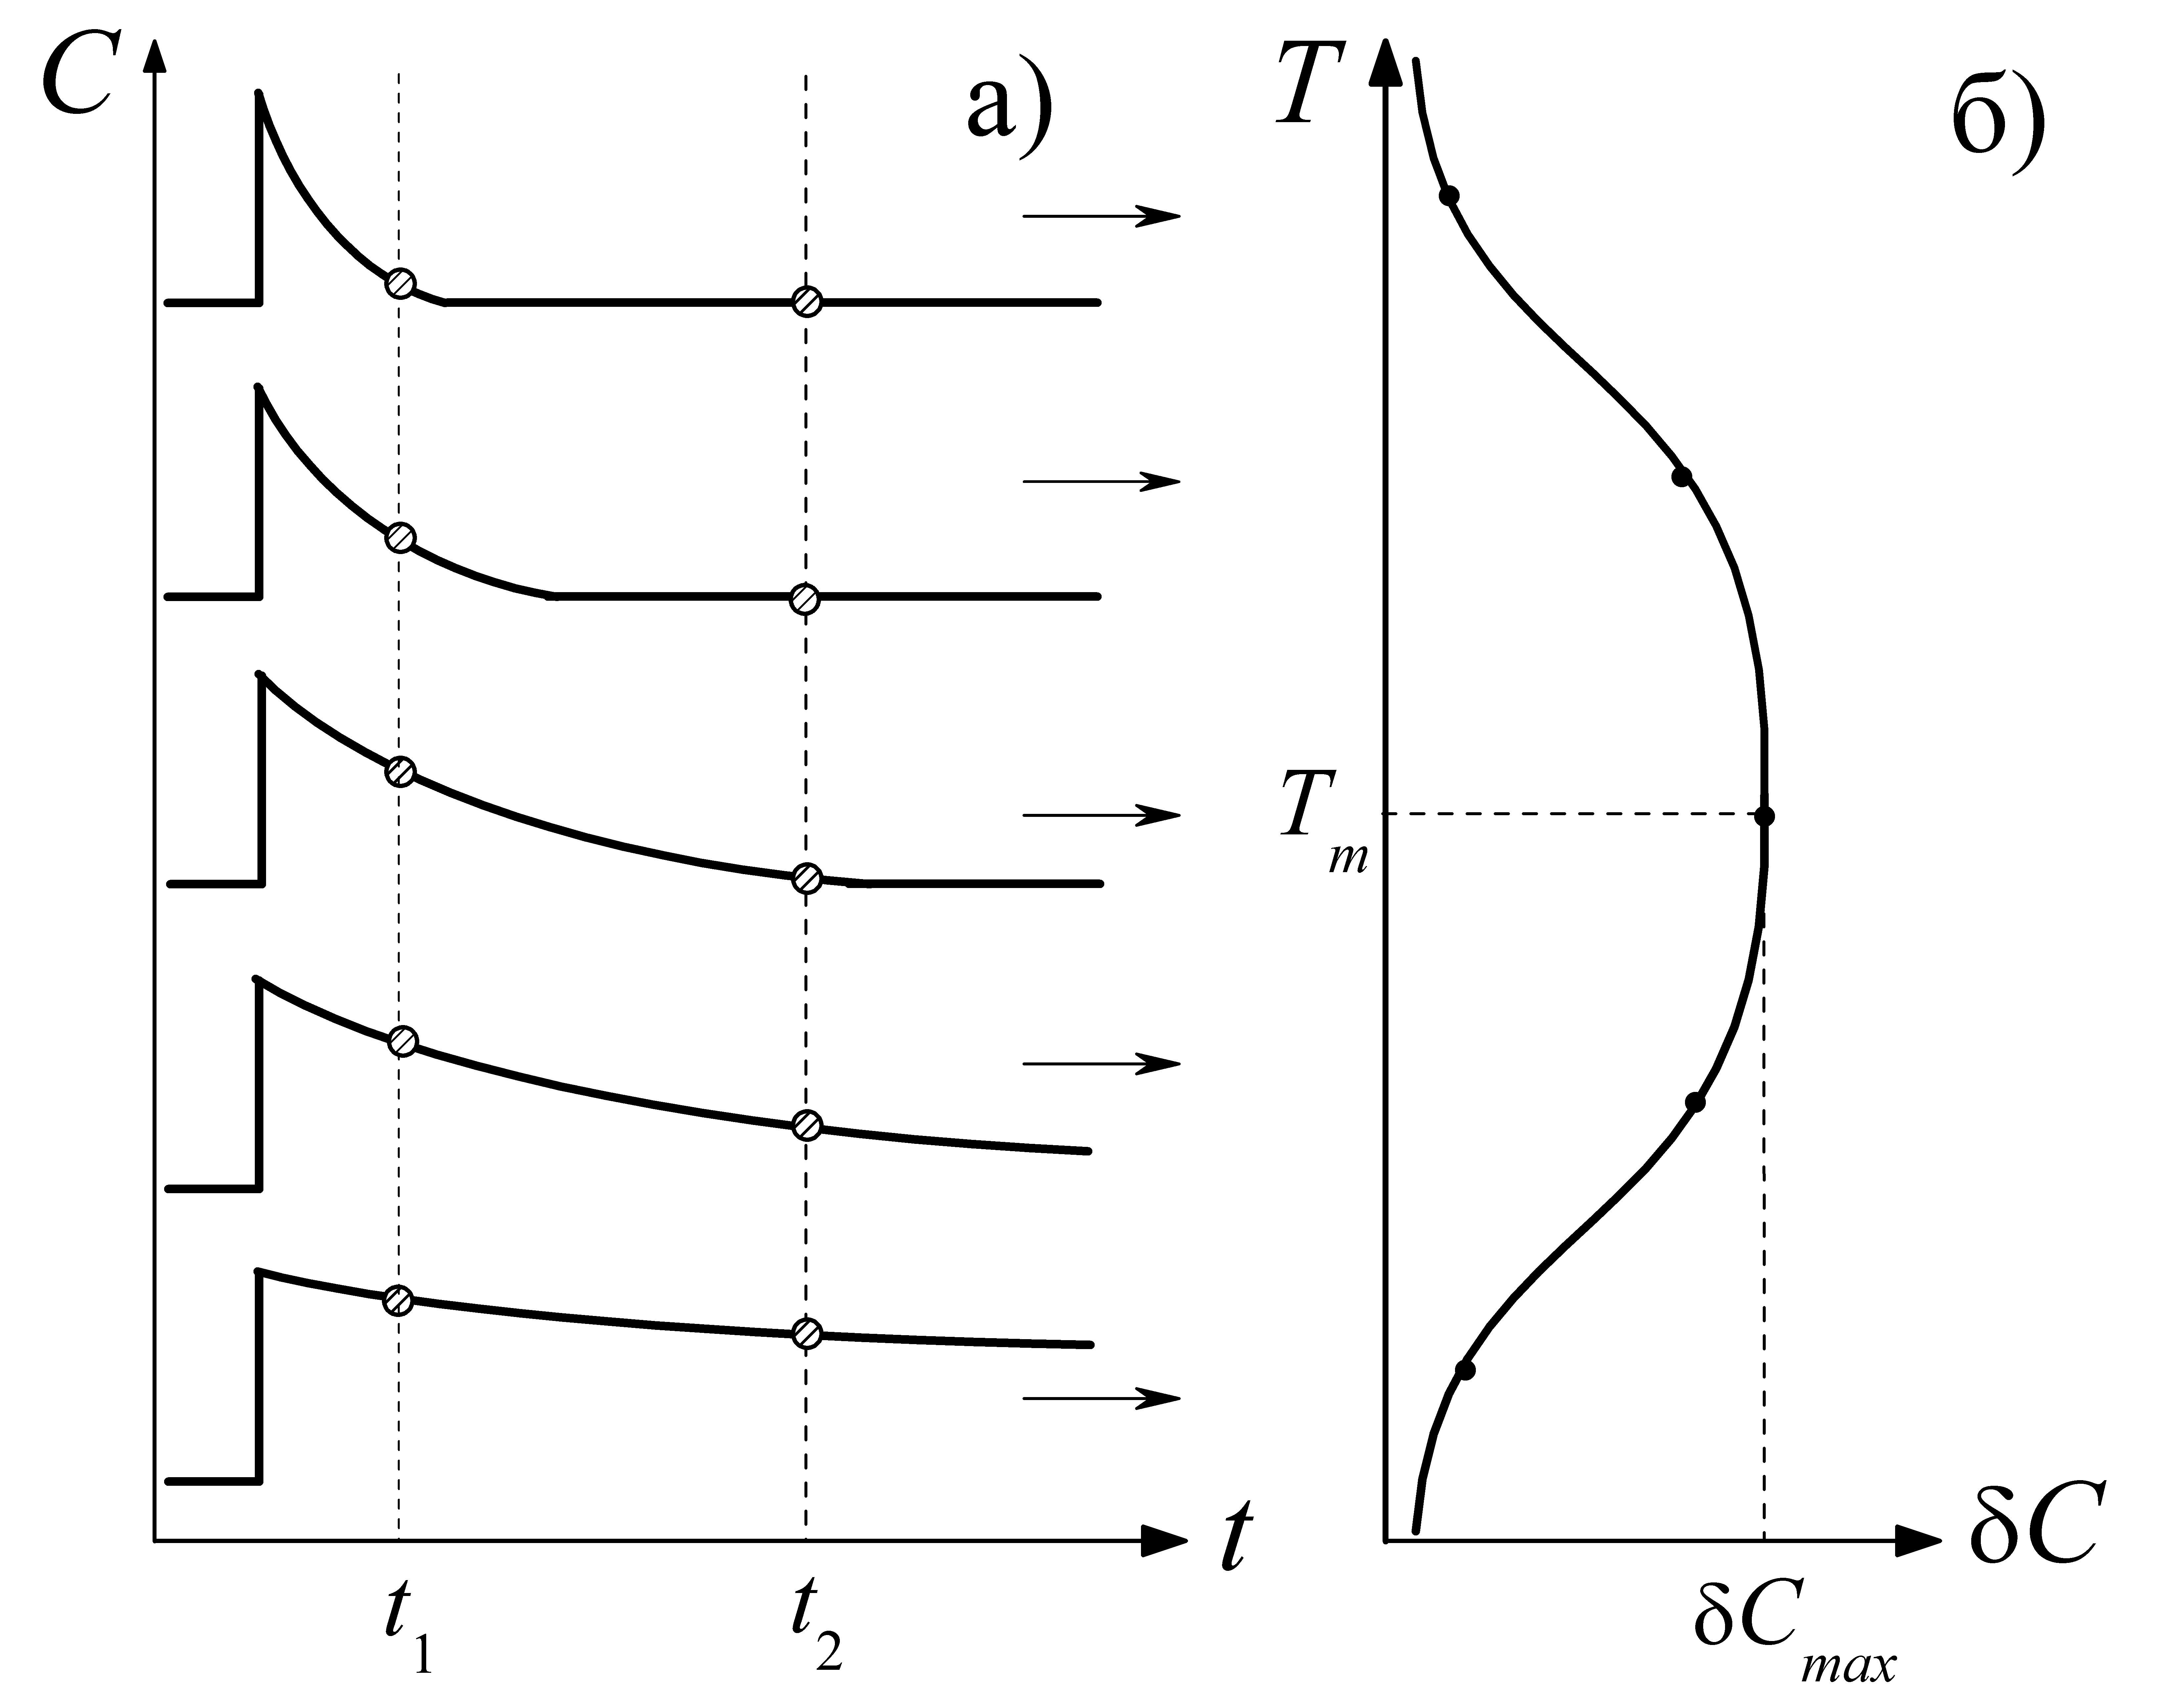
\includegraphics[width=0.65\textwidth]{Fig2_3}
\vspace{-3mm}
\caption{(а)~Характер релаксації ємності при різних температурах;
(б)~Спектр DLTS.
}
\vspace{-3mm}
\label{F23}
\end{figure}




Зазвичай напругу прикладають у імпульсному режимі, наприклад як показано на рис.\ref{F22},
вимірюючи ємність після закінчення так званого імпульсу заповнення тривалістю $t_p$
у два різних моменти часу ($t_1$ та $t_2$ на рисунку).
Саме різниця $\delta C=C(t_1)-C(t_2)$ і є сигналом DLTS.
Кінетика зміни ємності визначається процесом перезарядки дефектів
та за умов, зазначених вище, описується експоненційною залежністю:
\begin{equation}
\label{DLTSdelC}
C(t_1)-C(t_2)=\Delta C\,\left[\exp(-e_n t_1)-\exp(-e_n t_2)\right]\,,
\end{equation}
де
$e_n$ визначається виразом (\ref{en}).
Вимірювання проводяться в певному температурному діапазоні, залежність
$\delta C$ від температури називається спектром DLTS.
Швидкість емісії зростає з підвищення температури,
проте як при повільній (при низькій температурі) релаксації,
так і швидкі (при високій)
значення ємності в моменти вимірювання відрізняються мало --- див. рис.~\ref{F23},а.
Тому залежність $\delta C(T)$
характеризується наявністю максимуму (рис.~\ref{F23},б)
Відповідне екстремуму $\delta C(T)$ значення $e_{n,max}$ можна знайти з умови
\begin{equation*}
\left.\frac{d(\delta C)}{d e_n}\right|_{e_n=e_{n,max}}=0\,.
\end{equation*}
Враховуючи (\ref{DLTSdelC}), отримуємо
\begin{gather}
% \nonumber to remove numbering (before each equation)
  \frac{d\delta C}{d e_n} = \Delta C \left[-t_1\exp(-e_n t_1)+t_2\exp(-e_n t_2)\right]\,, \nonumber\\
  t_2\exp(-e_{n,max} t_2)-t_1\exp(-e_{n,max} t_1)= 0\,,\nonumber\\
  t_2\exp(-e_{n,max} t_2)= t_1\exp(-e_{n,max} t_1)\,, \nonumber\\
  \frac{t_2}{t_1} = \exp(-e_{n,max} (t_2-t_1))\,, \nonumber\\
  e_{n,max}=\frac{\ln\left(t_2/t_1\right)}{t_2-t_1}\,.\label{DLTSemax}
\end{gather}
Отже, якщо максимум залежності $\delta C(T)$ спостерігається при температурі $T_m$,
то має виконуватися рівність
\begin{equation}
\label{DLTSTmax}
\sigma_n(T_m)\,\upsilon_{th,n}\gamma_g N_C \exp\left(-\frac{E_C-E_t}{kT_m}\right)=\frac{\ln\left(t_2/t_1\right)}{t_2-t_1}\,.
\end{equation}

\begin{figure}[!b]
\center
\vspace{-5mm}
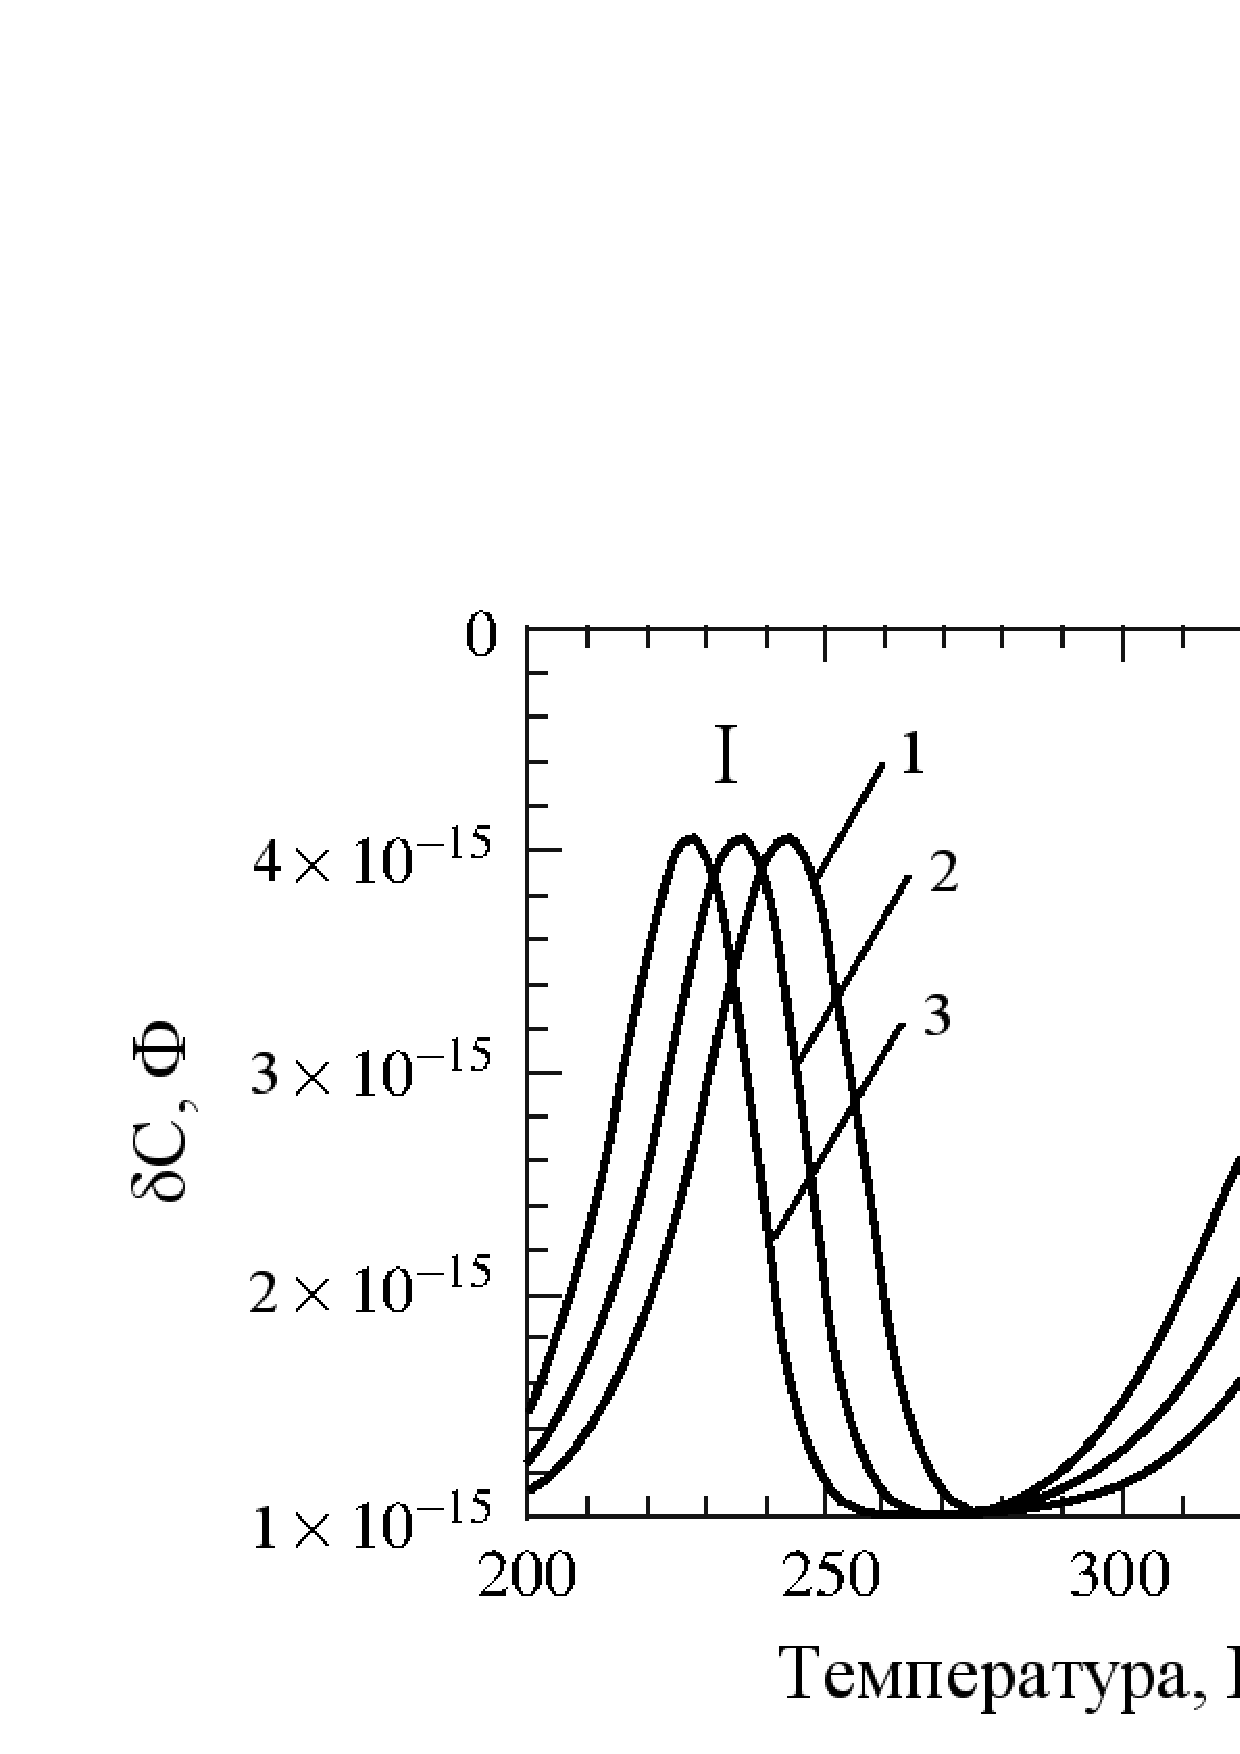
\includegraphics[width=0.65\textwidth]{Fig2_4}
\vspace{-3mm}
\caption{Розраховані спектри DLTS для різних значень $t_1$ та $t_2$.
Були використані значення
$t_1$, мс: 0,5 (крива 1), 1 (2), 2 (3);
$t_1$, мс: 1 (1), 2 (2), 4 (3);
$E_C-E_t$, еВ: 0,37 (для піку I), 0,6 (II);
$\sigma_n$, см$^2$: $10^{-15}$ (I), $5\cdot10^{-15}$ (II);
$N_t$, см$^{-3}$: $5\cdot10^{12}$ (I), $2\cdot10^{12}$ (II);
$C_0=4,9\cdot10^{-12}$~Ф, $N_d=10^{15}$~см$^{-3}$.
Рисунок адаптовано з \cite{Schroder2006}.
}
\vspace{-3mm}
\label{F24}
\end{figure}


Зрозуміло, що однієї рівності (\ref{DLTSTmax}) недостатньо,
щоб визначити дві невідомих характеристики дефекту $E_t$ та $\sigma_n(T_m)$.
Проте можна виміряти спектр DLTS при інших значеннях $t_1$ та $t_2$,
що призведе до зміщення положення максимуму --- відповідний випадок проілюстровано рисунком \ref{F24}.
Як наслідок, експериментально отримується набір температур $\left\{T_{m}\right\}$,
кожній з яких відповідає своя пара з набору  $\left\{(t_{1},t_{2})\right\}$.
Врахувавши співвідношення (\ref{enT}), можемо записати
\begin{equation}
\label{DLTSenT}
\ln\left(\frac{e_{n,max}}{T_m^2}\right)=\ln\left[\frac{\ln\left(t_2/t_1\right)}{\left(t_2-t_1\right)T_m^2}\right]=\ln\left(\beta\sigma_n\right)-\frac{E_C-E_t}{kT_m}\,.
\end{equation}
Тобто залежність $\ln(e_{n,max}\cdot T_m^{-2})$ від оберненої температури має бути прямою лінією,
нахил якої визначається положенням рівня у забороненій зоні, а точка перетину з вертикальною віссю ---
величиною поперечного перерізу захоплення.
Відхилення від лінійності та спотворення отриманих результатів може бути зумовлено температурною залежністю
$\sigma_n$, проте якщо її характер відомий, то цей ефект може бути враховано шляхом введення певних поправок.
Наприклад, якщо поперечний переріз захоплення є термоактивованою величиною (див.~(\ref{Sta})),
то нахил вказаної залежності буде дорівнюватиме не $(E_C-E_t)/k$, а $(E_C-E_t+E_{\sigma})/k$.




Якщо позначити $\delta C_{max}$ величину сигналу DLTS в максимумі,
то використовуючи вирази (\ref{DLTdelC*}), (\ref{DLTSdelC}) та (\ref{DLTSemax}) отримаємо
\begin{gather*}
% \nonumber to remove numbering (before each equation)
  \delta C_{max}=\frac{N_t\,C_0}{2N_D}\,\left\{\exp\left[-\frac{\ln\left(t_2/t_1\right)}{t_2-t_1}\cdot t_1\right]
     -\exp\left[-\frac{\ln\left(t_2/t_1\right)}{t_2-t_1}\cdot t_2\right]\right\}\,.\nonumber
\end{gather*}
Позначивши $b=t_2/t_1$ матимемо
\begin{gather}
% \nonumber to remove numbering (before each equation)
  \delta C_{max}=\frac{N_t\,C_0}{2N_D}\,\left\{\exp\left[-\frac{\ln\left(b\right)}{b-1}\right]
     -\exp\left[-\frac{\ln\left(b\right)}{1-b^{-1}} \right]\right\}\,,\nonumber\\
  \delta C_{max}=\frac{N_t\,C_0}{2N_D}\,\left\{\exp\left[-\frac{\ln\left(b\right)}{b-1}\right]
     -\exp\left[-\frac{b\ln\left(b\right)}{b-1} \right]\right\}\,,\nonumber\\
  \delta C_{max}=\frac{N_t\,C_0}{2N_D}\,\exp\left[-\frac{\ln\left(b\right)}{b-1}\right]\cdot
  \left\{1 -\left(\exp\left[-\frac{\ln\left(b\right)}{b-1} \right]\right)^{b-1}\right\}\,,\nonumber  \\
  \delta C_{max}=\frac{N_t\,C_0}{2N_D}\,\cdot b^{\frac{1}{1-b}}\cdot
  \left(1-\frac{1}{b}\right)\,,\nonumber     \\
    \delta C_{max}=\frac{N_t\,C_0}{2N_D}\,\cdot b^{\frac{1}{1-b}-1}\cdot \left(b-1\right)
                  =\frac{N_t\,C_0}{2N_D}\,\cdot b^{\frac{b}{1-b}}\cdot \left(b-1\right)\,,\nonumber \\
    N_t=\frac{2N_D\,\delta C_{max}b^{\frac{b}{b-1}}}{C_0\,(b-1)}\,.
\end{gather}
Тобто за висотою максимуму у спектрі DLTS можна  оцінити концентрацію дефектів.

Типова роздільна здатність при DLTS вимірюваннях $\delta C_{max}/C_0\approx(10^{-5}\div 10^{-4})$,
а отже метод дозволяє виявити дефекти з концентрацією порядку $(10^{-5}\div 10^{-4})N_D$.


При нерівномірному розподілі дефектів вираз (\ref{DLTdelC*}) перестає бути справедливим.
Водночас, варіюючи величину імпульсів заповнення та беручи до уваги відносні зміни ємності,
можна оцінити профіль концентрації дефектів:
\begin{equation}
\label{DLTSNt}
N_t(x)=\left(\frac{N_D^2W^2q}{\varepsilon\varepsilon_0}\right)\left(\frac{x-\lambda}{x}\right)\frac{d\left(\frac{\Delta C}{C}\right)}{dV}\,.
\end{equation}

Якщо у захопленні носіїв активно приймають участь декілька типів дефектів, то кожному
з них на спектрі DLTS буде відповідати свій пік.
Для випадку, коли параметри дефектів істотно відрізняються, ці піки легко розділяються
і DLTS дозволяє отримати параметри кожного з дефектів.


У вищеописаному традиційному DLTS--методі під час імпульсу заповнення заселеність пасток,
які переважно захоплюють неосновні носії заряду, не змінюється.
А отже, досліджуються рівні, які знаходяться, переважно, лише у одній половині  забороненої зони
(верхній для прикладу, що розглядався).
Але варіюючи знак імпульсів прикладеної до бар'єрної структури напруги можна
проводити дослідження різних типів дефектів, у тому числі й тих, які захоплюють носії заряду протилежних знаків.
Наприклад, для вивчення центрів захоплення неосновних носіїв може бути використаних режим,
ілюстрований рис.~\ref{F22}.
При прямому зміщенні інжектуються як основні, так і неосновні носії заряду та
відбувається зміна ємності збідненого прошарку внаслідок захоплення носіїв
обох знаків.
При наступному зворотному зміщенні процеси захоплення пригнічуються і
захоплені носії звільняються внаслідок термічної емісії.
Причому DLTS спектр у цьому випадку буде визначатися суперпозицією сигналів
від пасток обох типів.
Такий варіант досліджень нерідко називається інжекційна DLTS (inj--DLTS).

\begin{figure}[!b]
\center
\vspace{-5mm}
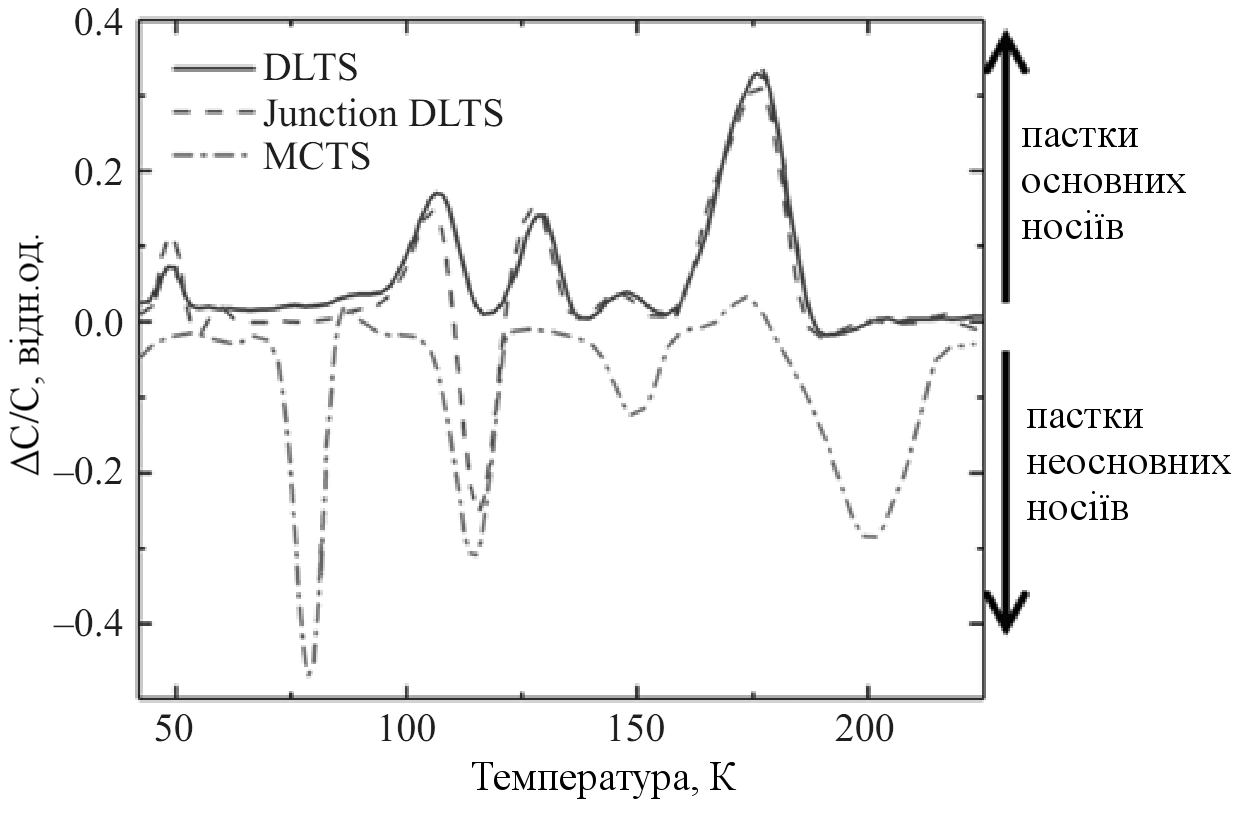
\includegraphics[width=0.75\textwidth]{Fig2_5}
\vspace{-3mm}
\caption{Спектри DLTS, inj--DLTS та MCTS.
Рисунок адаптовано з \cite{tuomisto2019}.
}
\vspace{-3mm}
\label{F25}
\end{figure}

Можна реалізувати випадок, коли в область просторового заряду вводяться лише неосновні носії.
Наприклад, подібна ситуація реалізується  при біполярній генерації носіїв за межами збідненого шару
на відстані порядку довжини дифузії від його межі.
Зокрема, цього можна досягти при освітленні структури з протилежного від бар'єру боку
і наступній дифузії в напрямку фронтальної площини.
Такий варіант DLTS називається MCTS (minority carrier transient spectroscopy).
В цьому випадку релаксація ємності та спектр матимуть протилежний знак.
Як приклад на рис.~\ref{F25} представлені спектри DLTS, інжекційної DLTS та MCTS.


За час застосування методу перехідної спектроскопії з'явилися й інші його модифікації.
Наприклад у методі ODLTS (optical deep--level transient spectroscopy), як і у традиційному DLTS,
вимірюється температурна залежність нестаціонарної ємності, проте стимуляція
процесів перезарядки глибоких центрів відбувається імпульсами світла, а не напруги.
Зазвичай енергія використаних фотонів менша ширини забороненої
зони ($0.5E_G<h\nu<E_G$),
освітлення відбувається при прикладеній зворотній напрузі.
У випадку напівпровідника $n$--типу, це викликає емісію електронів
з діркових пасток.
Після зняття оптичного імпульсу, пастки емітують дірки і спостерігається релаксація ємності.

У методі DLOS (deep--level optical spectroscopy) реєструється не температурний, а оптичний спектр нестаціонарної ємності.
При цьому існує два варіанти:
в методі термічної DLOS дослідження проводять при температурі, коли пастки внаслідок термічної емісії спустошені
і оптичним шляхом відбувається їх заповнення;
при оптичній DLOS використовується фотонно-стимульована емісія при знижених температурах,
коли вона переважає термічну.

Але чи не найцікавіщим варіантом є Laplace--DLTS (LDLTS) \cite{LDLTS2}.
В цьому випадку вимірювання релаксації ємності проводяться при постійній температурі,
після чого чисельно визначається спектр швидкості рекомбінації.
Процедура  подібна до зворотного перетворення Лапласа,
тобто знаходиться розв'язок рівняння
\begin{equation}
\label{DLTSLapl}
f(t)=\int_0^\infty F(s) e^{-st}ds\,.
\end{equation}
де
$f(t)$ --- виміряна часова залежність,
$F(s)$ --- шукана спектральна функція.
З математичної точки зору чи не найефективнішим вважається
метод регуляризації Тіхонова.
Якщо рівні дефектів розташовані дискретно і релаксація описується
однією чи декількома експонентами, то результуючий спектр
має складатися з $\delta$--подібних піків;
для неперервного енергетичного розподілу очікується широкий спектр.

Laplace--DLTS дозволив істотно підвищити роздільну здатність по енергії.
Наприклад, на рис.~\ref{F26} наведено приклад спектрів традиційного DLTS та LDLTS.
Якщо у першому випадку визначити наявність декількох рівнів
практично неможливо, то в другому присутність двох дефектів очевидна.

\begin{figure}[!t]
\center
\vspace{-5mm}
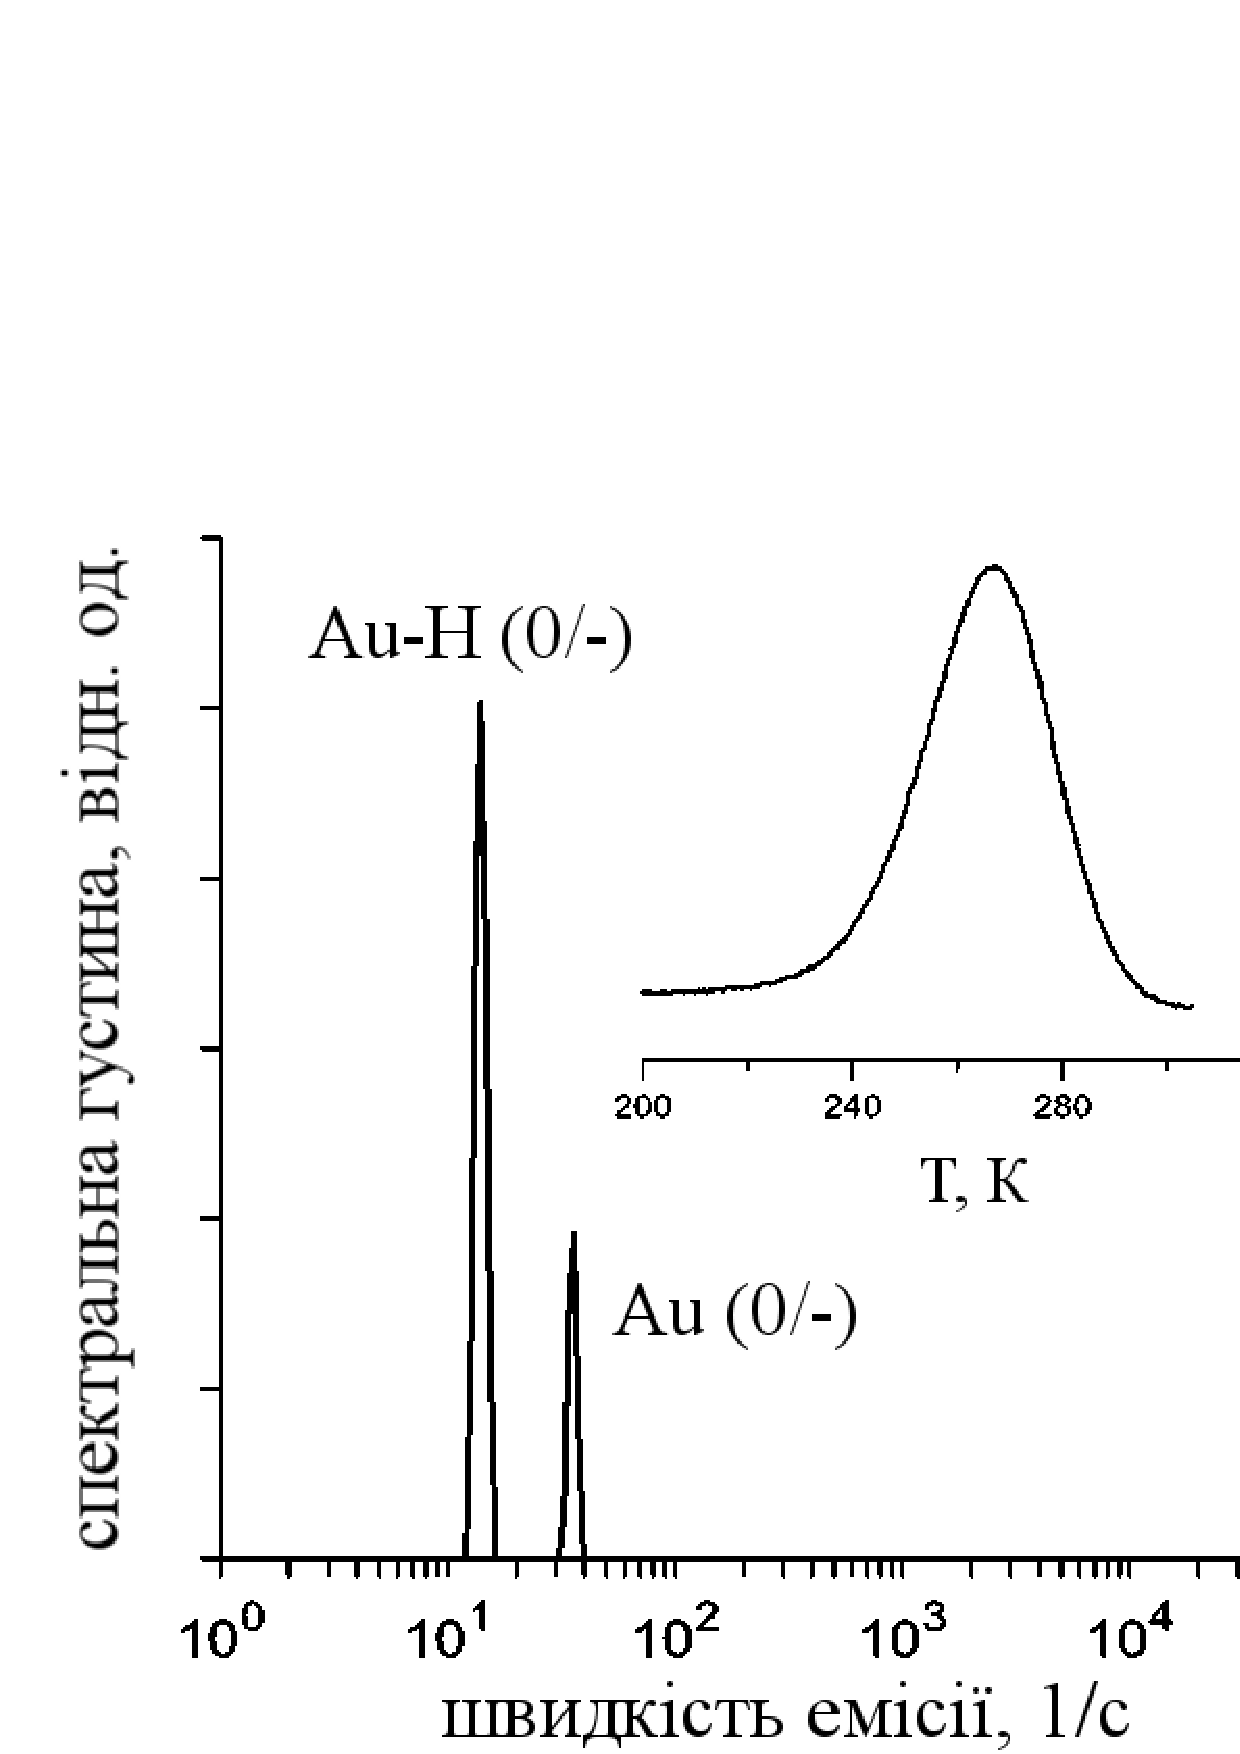
\includegraphics[width=0.65\textwidth]{Fig2_6}
\vspace{-3mm}
\caption{LDLTS спектр Si:(Au,H), виміряний при $T=260$~К.
Піки відповідають акцепторним рівням домішки золота та комплексу
золото--водень.
На вставці --- спектр традиційного DLTS того самого зразка.
Рисунок адаптовано з \cite{Deixler}.
}
\vspace{-3mm}
\label{F26}
\end{figure}

Крім названих варіантів існують й інші, такі як
D--DLTS (double correlation DLTS, використовуються імпульси заповнення з двома різними амплітудами),
СС--DLTS (constant capacitance DLTS, при емісії електронів ємність
залишається постійною завдяки зміні напруги зміщення),
I--DLTS (isothermal DLTS, аналізується похідна ємності по часу, отримана при постійній температурі),
С--DLTS (current DLTS, вимірюється температурна залежність нестаціонарного струму)
тощо.
